%%!
% @file main.tex
% @brief Master document assembling front matter, main chapters, and back matter.
%!TEX program = xelatex
\documentclass[12pt, a4paper, oneside]{report}

\usepackage{config/packages}
\usepackage{config/format}
%%!
% @file metadata.tex
% @brief Document metadata, institutional parameters, and contributor roster.

\university{TRƯỜNG ĐẠI HỌC GIAO THÔNG VẬN TẢI \n PHÂN HIỆU TẠI TP. HỒ CHÍ MINH}
\faculty{Bộ môn Công nghệ thông tin}
\institutionlogo{assets/logos/university_logo.pdf}

\subject{Tên môn học}
\reporttitle{Báo cáo bài tập lớn}
\subtitle{Tên đề tài nghiên cứu}

\supervisor{ThS. Trần Văn A}
\submissiondate{TP. Hồ Chí Minh, Ngày 10 Tháng 10 Năm 2026}

\addauthor{1}{Nguyễn Văn B}{65510200XX}{Nhiệm vụ 1}{20\%}
\addauthor{2}{Nguyễn Văn C}{66510710XX}{Nhiệm vụ 2}{30\%}
\addauthor{3}{Nguyễn Văn D}{66510710XX}{Nhiệm vụ 3}{25\%}
\addauthor{4}{Nguyễn Văn E}{66510710XX}{Nhiệm vụ 4}{15\%}
\addauthor{5}{Nguyễn Văn F}{66510710XX}{Nhiệm vụ 5}{10\%}

\studentclass{Mã lớp quản lý (Ví dụ: CQ.66.CNTT)}
\cohort{Khoá nhập học (Ví dụ: K66)}


\begin{document}

% 1. Main cover page
%%!
% @file 00_cover.tex
% @brief Title page template with institutional border, logo, and balanced metadata.
\begin{titlepage}
    \begin{tikzpicture}[remember picture, overlay]
        \draw[line width=3pt, color=black] 
            ([xshift=20mm, yshift=-20mm]current page.north west) 
            rectangle 
            ([xshift=-20mm, yshift=20mm]current page.south east);
    \end{tikzpicture}

    \vspace*{-4mm}

    \begin{center}
        {\fontsize{14pt}{18pt}\selectfont\bfseries \MakeUppercase{\theuniversity}\par}
        \vspace{4pt}
        {\fontsize{14pt}{18pt}\selectfont\bfseries \MakeUppercase{\thefaculty}\par}
        \vspace{24pt}
        \IfFileExists{\theinstitutionlogo}{%
            \includegraphics[width=3.6cm, height=3.6cm, keepaspectratio]{\theinstitutionlogo}%
        }{%
            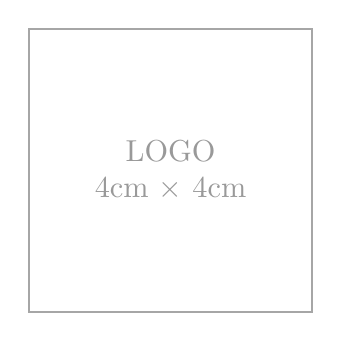
\begin{tikzpicture}
                \draw[thick, gray!70] (0,0) rectangle (3.6cm, 3.6cm);
                \node at (1.8cm, 1.8cm) [gray!80, align=center, font=\fontsize{11pt}{13pt}\selectfont] {LOGO\\4cm $\times$ 4cm};
            \end{tikzpicture}
        }
        \par
        \vspace{14pt}

        {\fontsize{14pt}{18pt}\selectfont\bfseries \MakeUppercase{\thesubject}\par}
        \vspace{16pt}

        {\fontsize{14pt}{18pt}\selectfont\bfseries \MakeUppercase{\thereporttitle}\par}
        \ifx\thesubtitle\empty\relax\else
            \vspace{6pt}
            {\fontsize{13pt}{16pt}\selectfont\bfseries \thesubtitle\par}
        \fi
    \end{center}

    \vspace*{\fill}

    \noindent\renderauthorblock

    \vspace*{\fill}

    \begin{center}
        {\fontsize{14pt}{18pt}\selectfont \thesubmissiondate\par}
    \end{center}
    \vspace*{24pt}
\end{titlepage}


% 2. Sub cover page
%%!
% @file 00_subcover.tex
% @brief Sub-cover (inside title page) template with formal double-border frame.

\begin{titlepage}
    \begin{tikzpicture}[remember picture, overlay]
        % Khung vien ngoai (1.5pt)
        \draw[line width=1.5pt, color=black] 
            ([xshift=20mm, yshift=-20mm]current page.north west) 
            rectangle 
            ([xshift=-20mm, yshift=20mm]current page.south east);
        % Khung vien trong (0.5pt) cach khung ngoai 1.5mm
        \draw[line width=0.5pt, color=black] 
            ([xshift=21.5mm, yshift=-21.5mm]current page.north west) 
            rectangle 
            ([xshift=-21.5mm, yshift=21.5mm]current page.south east);
    \end{tikzpicture}

    \vspace*{-4mm}

    \begin{center}
        {\fontsize{14pt}{18pt}\selectfont\bfseries \MakeUppercase{\theuniversity}\par}
        \vspace{4pt}
        {\fontsize{14pt}{18pt}\selectfont\bfseries \MakeUppercase{\thefaculty}\par}
        \vspace{24pt}
        \IfFileExists{\theinstitutionlogo}{%
            \includegraphics[width=3.6cm, height=3.6cm, keepaspectratio]{\theinstitutionlogo}%
        }{%
            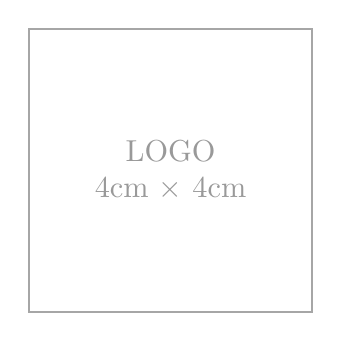
\begin{tikzpicture}
                \draw[thick, gray!70] (0,0) rectangle (3.6cm, 3.6cm);
                \node at (1.8cm, 1.8cm) [gray!80, align=center, font=\fontsize{11pt}{13pt}\selectfont] {LOGO\\4cm $\times$ 4cm};
            \end{tikzpicture}
        }
        \par
        \vspace{14pt}

        {\fontsize{14pt}{18pt}\selectfont\bfseries \MakeUppercase{\thesubject}\par}
        \vspace{16pt}

        {\fontsize{14pt}{18pt}\selectfont\bfseries \MakeUppercase{\thereporttitle}\par}
        \ifx\thesubtitle\empty\relax\else
            \vspace{6pt}
            {\fontsize{13pt}{16pt}\selectfont\bfseries \thesubtitle\par}
        \fi
    \end{center}

    \vspace*{\fill}

    \noindent\renderauthorblock

    \vspace*{\fill}

    \begin{center}
        {\fontsize{14pt}{18pt}\selectfont \thesubmissiondate\par}
    \end{center}
    \vspace*{24pt}
\end{titlepage}


% 3. Lecturer review form (without page numbering)
%%!
% @file 01_lecturer_review.tex
% @brief Advisor feedback and assessment sheet without page numbering.

\chapter*{NHẬN XÉT CỦA GIẢNG VIÊN HƯỚNG DẪN}
\thispagestyle{empty}

\noindent\dotfill\par
\noindent\dotfill\par
\noindent\dotfill\par
\noindent\dotfill\par
\noindent\dotfill\par
\noindent\dotfill\par

\vspace{1.5cm}
\begin{flushright}
    \textit{Ngày \dots\dots\ tháng \dots\dots\ năm 20\dots}\\[0.4cm]
    \begin{tabular}{@{}c@{}}
        \textbf{Chữ ký giảng viên hướng dẫn} \\[2.0cm]
        \textbf{\thesupervisor}
    \end{tabular}
\end{flushright}


\newpage
\pagenumbering{roman}

% 4. Affidavit of originality and authenticity
%%!
% @file 03_affirmation.tex
% @brief Authors' academic integrity and affirmation declaration.

\chapter*{LỜI CAM ĐOAN}
\addcontentsline{toc}{chapter}{Lời cam đoan}

Chúng tôi xin cam đoan rằng đồ án / báo cáo bài tập lớn này là công trình nghiên cứu và thực hiện độc lập của nhóm chúng tôi dưới sự hướng dẫn khoa học của cán bộ hướng dẫn.

Mọi số liệu, hình ảnh, bảng biểu và kết quả trình bày trong báo cáo là hoàn toàn trung thực và chưa từng được công bố trong bất kỳ công trình nghiên cứu nào khác nhằm mục đích nhận học vị hoặc điểm thưởng. Các nội dung tham khảo, kế thừa từ các công trình nghiên cứu khác đều đã được trích dẫn nguồn gốc rõ ràng, đầy đủ theo đúng chuẩn mực học thuật quy định.

Nếu có bất kỳ sự gian lận hoặc vi phạm quy chế học thuật nào, nhóm chúng tôi xin hoàn toàn chịu trách nhiệm trước Hội đồng đánh giá và Nhà trường.

\vspace{1.5cm}
\begin{flushright}
    \textit{\thesubmissiondate}\\[0.4cm]
    \begin{tabular}{@{}c@{}}
        \textbf{Đại diện nhóm sinh viên thực hiện}\\[2.0cm]
        \textbf{\getauthorname{1}}
    \end{tabular}
\end{flushright}


% 5. Acknowledgments
%%!
% @file 04_acknowledgments.tex
% @brief Acknowledgments acknowledging advisor, faculty, and supporters.

\chapter*{LỜI CẢM ƠN}
\addcontentsline{toc}{chapter}{Lời cảm ơn}

Lời đầu tiên, nhóm tác giả xin gửi lời cảm ơn chân thành và sâu sắc nhất tới cán bộ hướng dẫn, \thesupervisor, người đã luôn tận tình định hướng, chia sẻ kiến thức chuyên môn và đưa ra những đóng góp quý báu trong suốt quá trình nhóm nghiên cứu và triển khai đề tài.

Chúng tôi cũng xin trân trọng cảm ơn Ban giám hiệu , Ban chủ nhiệm cùng toàn thể quý thầy cô thuộc \thefaculty đã tạo điều kiện học tập tốt nhất, truyền đạt nền tảng kiến thức vững chắc và hỗ trợ cơ sở vật chất kỹ thuật trong suốt thời gian học tập tại trường.

Cuối cùng, chúng tôi xin gửi lời cảm ơn tới gia đình, bạn bè và các bạn sinh viên đã luôn động viên, khích lệ và đồng hành cùng chúng tôi để hoàn thành tốt bản báo cáo này.


% 6. Table of task assignment
%%!
% @file 02_task_assignment.tex
% @brief Task assignment board mapping team members to their responsibilities.

\chapter*{BẢNG PHÂN CÔNG NHIỆM VỤ}
\addcontentsline{toc}{chapter}{Bảng phân công nhiệm vụ}

\begin{table}[h!]
    \centering
    \begin{tabularx}{\textwidth}{|C{2.6cm}|L{3.2cm}|Y|C{2.0cm}|C{2.0cm}|}
        \hline
        \thcell{MSSV}   & \thcell{Họ và tên SV} & \thcell{Nhiệm vụ được phân công} & \thcell{Mức đóng góp}      & \thcell{Ký tên}   \\ \hline
        \getauthorid{1} & \getauthorname{1}     & \getauthortask{1}    & \getauthorcontrib{1} & \rule{0pt}{0.8cm} \\ \hline
        \getauthorid{2} & \getauthorname{2}     & \getauthortask{2}    & \getauthorcontrib{2} & \rule{0pt}{0.8cm} \\ \hline
        \getauthorid{3} & \getauthorname{3}     & \getauthortask{3}    & \getauthorcontrib{3} & \rule{0pt}{0.8cm} \\ \hline
        \getauthorid{4} & \getauthorname{4}     & \getauthortask{4}    & \getauthorcontrib{4} & \rule{0pt}{0.8cm} \\ \hline
        \getauthorid{5} & \getauthorname{5}     & \getauthortask{5}    & \getauthorcontrib{5} & \rule{0pt}{0.8cm} \\ \hline
    \end{tabularx}
\end{table}


% 7. Table of contents, list of figures, and list of tables
%%!
% @file 05_lists.tex
% @brief Front matter index pages: Table of Contents, Figures, Tables, Listings, and Abbreviations.

\renewcommand{\contentsname}{MỤC LỤC}
\tableofcontents
\newpage

\renewcommand{\listfigurename}{DANH MỤC HÌNH VẼ}
\listoffigures
\addcontentsline{toc}{chapter}{Danh mục hình vẽ}
\newpage

\renewcommand{\listtablename}{DANH MỤC BẢNG BIỂU}
\listoftables
\addcontentsline{toc}{chapter}{Danh mục bảng biểu}
\newpage

\renewcommand{\lstlistlistingname}{DANH MỤC ĐOẠN MÃ}
\lstlistoflistings
\addcontentsline{toc}{chapter}{Danh mục đoạn mã}
\newpage

%%!
% @file abbreviations.tex
% @brief Abbreviations list formatted as a three-column reference table.

\chapter*{DANH MỤC TỪ VIẾT TẮT}
\addcontentsline{toc}{chapter}{Danh mục từ viết tắt}

\begin{table}[h!]
    \centering
    \begin{tabularx}{\textwidth}{|C{2.8cm}|L{6.2cm}|Y|}
        \hline
        \thcell{Từ viết tắt} & \thcell{Từ đầy đủ}                             & \thcell{Nghĩa tiếng Việt}                 \\ \hline
        AI                   & Artificial Intelligence                        & Trí tuệ nhân tạo                          \\ \hline
        API                  & Application Programming Interface              & Giao diện lập trình ứng dụng              \\ \hline
        CI/CD                & Continuous Integration / Continuous Deployment & Tích hợp liên tục và Triển khai liên tục \\ \hline
        CRUD                 & Create, Read, Update, Delete                   & Khởi tạo, Đọc, Cập nhật, Xóa             \\ \hline
        DBMS                 & Database Management System                     & Hệ quản trị cơ sở dữ liệu                 \\ \hline
        HTTP                 & Hypertext Transfer Protocol                    & Giao thức truyền tải siêu văn bản        \\ \hline
        OOP                  & Object-Oriented Programming                    & Lập trình hướng đối tượng                 \\ \hline
        OS                   & Operating System                               & Hệ điều hành                              \\ \hline
        REST                 & Representational State Transfer                & Chuyển giao trạng thái đại diện          \\ \hline
        UI                   & User Interface                                 & Giao diện người dùng                      \\ \hline
        UX                   & User Experience                                & Trải nghiệm người dùng                    \\ \hline
    \end{tabularx}
\end{table}

\newpage


\newpage
\pagenumbering{arabic}
%%!
% @file 01_introduction.tex
% @brief Template for Chapter 1 demonstrating heading hierarchy, lists, tables, figures, and code.

\chapter{Tiêu đề chương 1}
\label{chap:chapter_1}

Đây là nội dung mở đầu của chương 1 trong bản mẫu báo cáo. Đoạn văn bản này minh họa định dạng chuẩn với cỡ chữ 13pt, khoảng cách giãn dòng 1.5 và thụt đầu dòng 1.25cm theo quy định kỹ thuật \cite{doe2023}. Nội dung mẫu có thể được thay thế bằng phần giới thiệu tổng quan, bối cảnh thực hiện hoặc mục tiêu nghiên cứu của đề tài.

Lorem ipsum dolor sit amet, consectetur adipiscing elit. Sed do eiusmod tempor incididunt ut labore et dolore magna aliqua. Ut enim ad minim veniam, quis nostrud exercitation ullamco laboris nisi ut aliquip ex ea commodo consequat \cite{newman2021}.

\section{Tiêu đề mục 1.1}
\label{sec:section_1_1}

Nội dung chi tiết của mục 1.1 trình bày cơ sở lý luận, bối cảnh hoặc các vấn đề trọng tâm liên quan đến nội dung chương 1. Dưới đây là các tiểu mục được phân cấp chi tiết.

\subsection{Tiêu đề mục 1.1.1}
\label{subsec:subsection_1_1_1}

Nội dung minh họa của mục 1.1.1. Đoạn này minh họa cách trình bày danh sách hoa thị đa cấp theo chuẩn định dạng kỹ thuật:

\begin{itemize}
    \item Nội dung danh sách cấp 1 -- Mục thứ nhất (sử dụng dấu gạch ngang, khoảng cách lề trái chuẩn).
    \item Nội dung danh sách cấp 1 -- Mục thứ hai với các ý chi tiết bên trong:
          \begin{itemize}
              \item Nội dung danh sách cấp 2 -- Chi tiết 2.1 (sử dụng ký hiệu dấu cộng, thụt đầu dòng 1.25cm).
              \item Nội dung danh sách cấp 2 -- Chi tiết 2.2.
          \end{itemize}
    \item Nội dung danh sách cấp 1 -- Mục thứ ba.
\end{itemize}

\subsubsection{Tiêu đề mục 1.1.1.1}
\label{subsubsec:subsubsection_1_1_1_1}

Nội dung minh họa cấp đề mục thứ 4 (Sub-subsection) với tiền tố số 4 cấp. Theo đặc tả mẫu, cấp này chỉ hiển thị trong nội dung chính và tự động không xuất hiện trong Mục lục để đảm bảo tính tinh gọn của tài liệu.

\section{Tiêu đề mục 1.2}
\label{sec:section_1_2}

Mục này minh họa quy cách trình bày các đối tượng nổi (floats) bao gồm bảng biểu và hình vẽ, cùng cơ chế tham chiếu chéo tự động. Bảng \ref{tab:sample_table} minh họa bảng dữ liệu mẫu có đệm 4pt trên và dưới.

%%!
% @brief Example table demonstrating the use of tabularx and custom column types in LaTeX.

\begin{table}[h!]
    \caption{Tiêu đề bảng 1.1}
    \label{tab:sample_table}
    \centering
    \begin{tabularx}{\textwidth}{|C{1.5cm}|Y|C{3.0cm}|C{3.0cm}|}
        \hline
        \thcell{STT} & \thcell{Tiêu chí đánh giá mẫu} & \thcell{Thông số A} & \thcell{Thông số B} \\ \hline
        1            & Dữ liệu thử nghiệm mẫu số 01   & 100                 & 200                 \\ \hline
        2            & Dữ liệu thử nghiệm mẫu số 02   & 300                 & 400                 \\ \hline
        3            & Dữ liệu thử nghiệm mẫu số 03   & 500                 & 600                 \\ \hline
    \end{tabularx}
\end{table}

Bên cạnh bảng biểu, Hình \ref{fig:sample_figure} minh họa một sơ đồ khối kỹ thuật được vẽ trực tiếp bằng gói lệnh TikZ với chú thích căn giữa bên dưới hình ảnh.

\begin{figure}[h!]
    \centering
    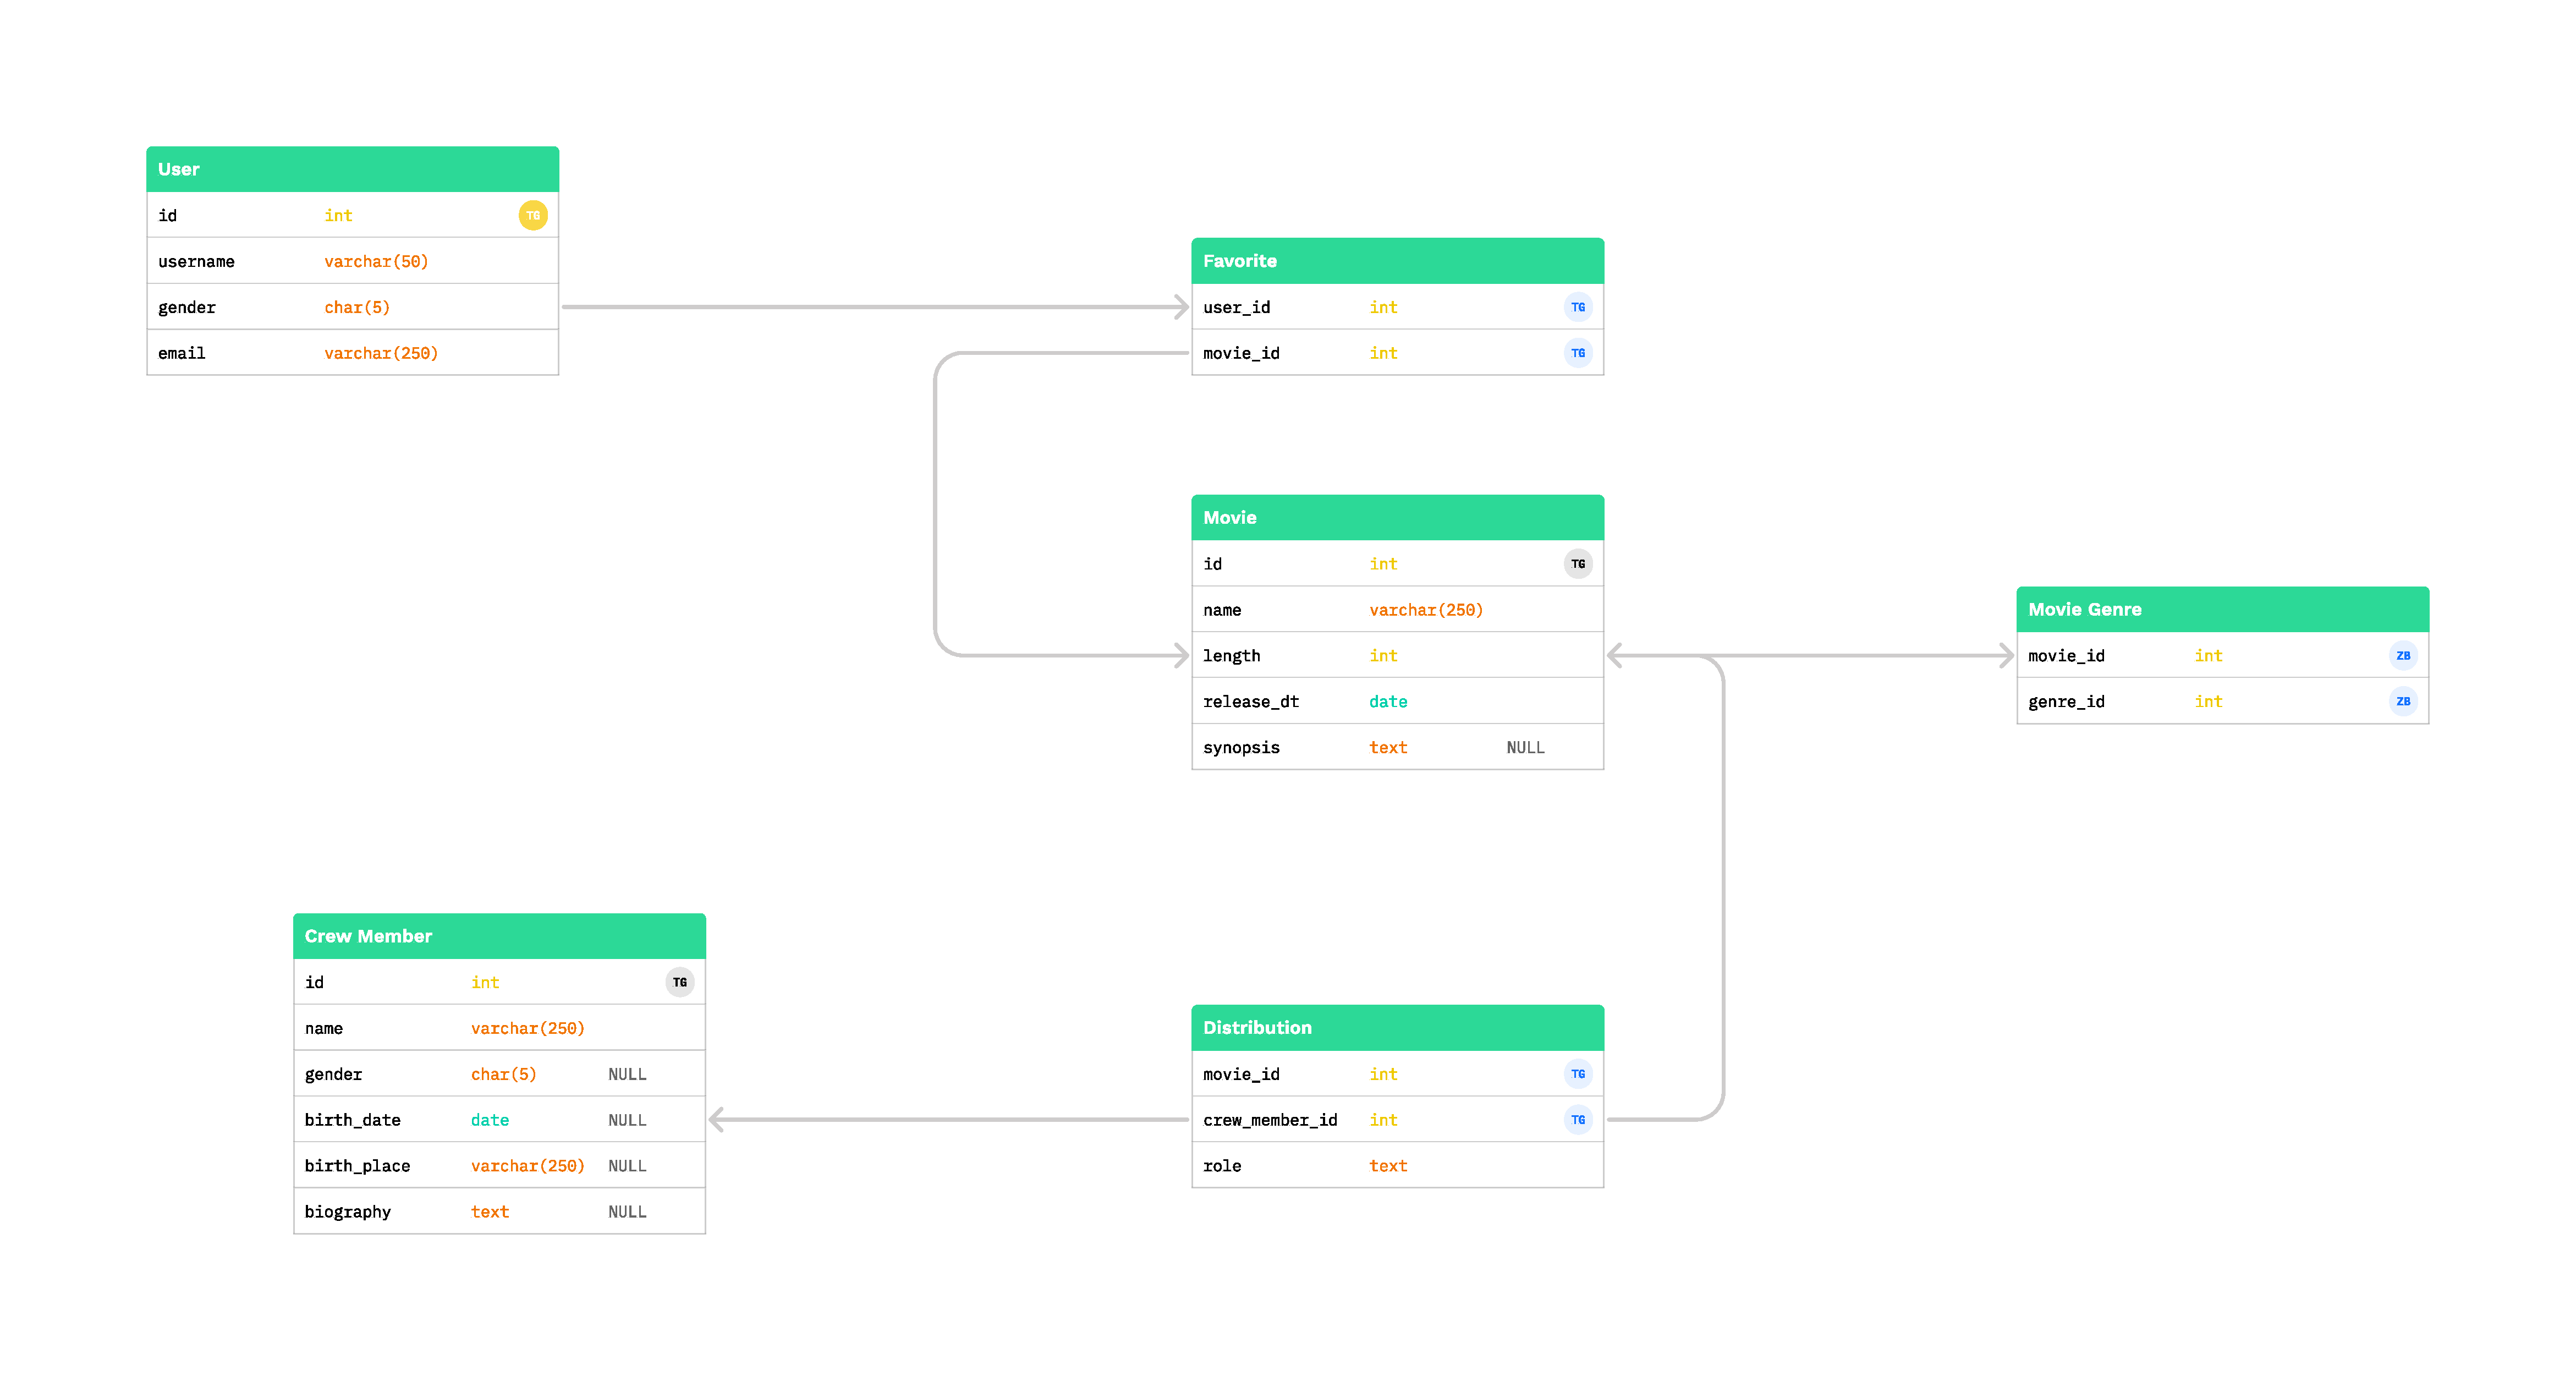
\includegraphics[width=\textwidth, height=0.7\textheight, keepaspectratio]{assets/figures/ch01/example_figure.pdf}
    \caption{Tiêu đề hình 1.1}
    \label{fig:sample_figure}
\end{figure}

\section{Tiêu đề mục 1.3}
\label{sec:section_1_3}

Đoạn mã sau minh họa cách trình bày khối mã nguồn hệ thống với định dạng hộp viền đơn, cỡ chữ 10pt phông Inconsolata, như được hiển thị tại Đoạn mã \ref{lst:sample_code}.

\begin{lstlisting}[language=Python, caption={Tiêu đề đoạn mã 1.1}, label={lst:sample_code}]
def example_function(param_a: int, param_b: int) -> int:
    """Tinh tong hai so nguyen va tra ve ket qua."""
    result = param_a + param_b
    return result

if __name__ == "__main__":
    output = example_function(10, 20)
    print(f"Ket qua tinh toan: {output}")
\end{lstlisting}

%%!
% @file 02_literature_review.tex
% @brief Template for Chapter 2 demonstrating inline and display mathematical formulas.

\chapter{Tiêu đề chương 2}
\label{chap:chapter_2}

Nội dung mở đầu của chương 2 trình bày tổng quan các nghiên cứu liên quan, cơ sở lý thuyết nền tảng và các mô hình toán học hoặc kỹ thuật ứng dụng trong phạm vi đề tài nghiên cứu.

Duis aute irure dolor in reprehenderit in voluptate velit esse cillum dolore eu fugiat nulla pariatur. Excepteur sint occaecat cupidatat non proident, sunt in culpa qui officia deserunt mollit anim id est laborum.

\section{Tiêu đề mục 2.1}
\label{sec:section_2_1}

Nội dung chi tiết của mục 2.1 tổng hợp các lý thuyết chính, phương pháp luận và các mô hình toán học nền tảng. Dưới đây là các định dạng công thức toán học mẫu theo chuẩn học thuật.

\subsection{Tiêu đề mục 2.1.1}
\label{subsec:subsection_2_1_1}

Tiểu mục này minh họa công thức toán học trong dòng văn bản (\textit{inline math}) và công thức toán học hiển thị riêng biệt (\textit{display math}).

Trong dòng văn bản, ta có thể biểu diễn các đại lượng như biến số $x \in \mathbb{R}$, vector đặc trưng $\mathbf{x} = [x_1, x_2, \dots, x_n]^T \in \mathbb{R}^n$, hay hàm mục tiêu $f(x) = \frac{1}{1 + e^{-x}}$. Đánh giá độ phức tạp tính toán của thuật toán cũng được thể hiện rõ ràng qua ký hiệu Big-$\mathcal{O}$ như $\mathcal{O}(n \log n)$ với điều kiện ràng buộc sai số $\epsilon \le 10^{-4}$.

Đối với các công thức trọng tâm, ta sử dụng môi trường công thức hiển thị riêng dòng (\textit{display math}) có đánh số tự động để phục vụ việc tham chiếu chéo. Công thức \eqref{eq:sample_sigmoid} biểu diễn hàm kích hoạt chuẩn:

\begin{equation}
    \label{eq:sample_sigmoid}
    \sigma(z) = \frac{1}{1 + e^{-z}} = \frac{e^z}{e^z + 1}, \quad \forall z \in \mathbb{R}
\end{equation}

Khi cần trình bày hệ công thức hoặc bài toán tối ưu nhiều bước có căn chỉnh dấu bằng, môi trường \texttt{align} được sử dụng như minh họa trong hệ thức \eqref{eq:sample_loss} và \eqref{eq:sample_gradient}:

\begin{align}
    \label{eq:sample_loss}
    \mathcal{L}(\mathbf{w}) &= -\frac{1}{N} \sum_{i=1}^{N} \left[ y_i \ln(\hat{y}_i) + (1 - y_i)\ln(1 - \hat{y}_i) \right] + \frac{\lambda}{2} \|\mathbf{w}\|_2^2, \\
    \label{eq:sample_gradient}
    \nabla_{\mathbf{w}} \mathcal{L}(\mathbf{w}) &= \frac{1}{N} \sum_{i=1}^{N} (\hat{y}_i - y_i) \mathbf{x}_i + \lambda \mathbf{w}.
\end{align}

Ngoài ra, trường hợp cần hiển thị công thức ma trận không đánh số, ta có thể sử dụng môi trường dấu ngoặc vuông \texttt{\textbackslash[ \dots \textbackslash]} kết hợp môi trường \texttt{bmatrix}:

\[
    \mathbf{A} = \begin{bmatrix}
        a_{11} & a_{12} & \dots  & a_{1n} \\
        a_{21} & a_{22} & \dots  & a_{2n} \\
        \vdots & \vdots & \ddots & \vdots \\
        a_{m1} & a_{m2} & \dots  & a_{mn}
    \end{bmatrix} \in \mathbb{R}^{m \times n}
\]

\section{Tiêu đề mục 2.2}
\label{sec:section_2_2}

Nội dung chi tiết của mục 2.2 so sánh, đánh giá đối chiếu giữa các phương pháp tiếp cận khác nhau nhằm định hình giải pháp tối ưu cho đề tài nghiên cứu.

%%!
% @file 03_system_architecture.tex
% @brief Template for Chapter 3.

\chapter{Tiêu đề chương 3}
\label{chap:chapter_3}

Chương 3 trình bày chi tiết về thiết kế hệ thống, mô hình kiến trúc tổng thể, các luồng tương tác nghiệp vụ và đặc tả giao diện giữa các thành phần phần mềm.

Sed ut perspiciatis unde omnis iste natus error sit voluptatem accusantium doloremque laudantium, totam rem aperiam, eaque ipsa quae ab illo inventore veritatis et quasi architecto beatae vitae dicta sunt explicabo.

\section{Tiêu đề mục 3.1}
\label{sec:section_3_1}

Nội dung chi tiết của mục 3.1 mô tả kiến trúc phân tầng, phân chia nhiệm vụ và trách nhiệm của từng phân hệ trong cấu trúc tổng quan.

\subsection{Tiêu đề mục 3.1.1}
\label{subsec:subsection_3_1_1}

Nội dung chi tiết của tiểu mục 3.1.1 đặc tả các giao thức truyền tải, chuẩn giao tiếp dữ liệu và cơ chế bảo mật trao đổi thông tin.

\section{Tiêu đề mục 3.2}
\label{sec:section_3_2}

Nội dung chi tiết của mục 3.2 mô tả lược đồ thiết kế dữ liệu, cấu trúc bảng quan hệ hoặc các mô hình lưu trữ phi cấu trúc phục vụ đề tài.

%%!
% @file 04_implementation.tex
% @brief Template for Chapter 4.

\chapter{Tiêu đề chương 4}
\label{chap:chapter_4}

Chương 4 tập trung vào quy trình hiện thực hóa giải pháp kỹ thuật, triển khai cài đặt các mô-đun chức năng và tiến hành thử nghiệm đánh giá hiệu quả thực tế.

Nemo enim ipsam voluptatem quia voluptas sit aspernatur aut odit aut fugit, sed quia consequuntur magni dolores eos qui ratione voluptatem sequi nesciunt. Neque porro quisquam est, qui dolorem ipsum quia dolor sit amet.

\section{Tiêu đề mục 4.1}
\label{sec:section_4_1}

Nội dung chi tiết của mục 4.1 mô tả môi trường thực thi, công cụ phát triển phần mềm, thư viện liên kết và cấu hình hạ tầng kiểm thử.

\subsection{Tiêu đề mục 4.1.1}
\label{subsec:subsection_4_1_1}

Nội dung chi tiết của tiểu mục 4.1.1 trình bày các kịch bản kiểm thử đơn vị, kiểm thử tích hợp và tiêu chí đánh giá độ tin cậy của hệ thống.

\section{Tiêu đề mục 4.2}
\label{sec:section_4_2}

Nội dung chi tiết của mục 4.2 tổng hợp và phân tích các chỉ số kết quả kiểm thử tải, hiệu năng xử lý và tỷ lệ hoàn thành tác vụ.

%%!
% @file 05_conclusion.tex
% @brief Template for Chapter 5 (Conclusions and Future Work).

\chapter{Tiêu đề chương 5}
\label{chap:chapter_5}

Chương cuối tổng kết lại các mục tiêu đã hoàn thành của đề tài nghiên cứu, các kết quả đạt được, hạn chế còn tồn tại và đề xuất các hướng phát triển mở rộng trong tương lai.

Lorem ipsum dolor sit amet, consectetur adipiscing elit. Nullam nonummy aliquam ante. Etiam elementum pellentesque sapien. Proin sodales libero eget ante. Nulla turpis magna, cursus sit amet, suscipit a, interdum id, felis.

\section{Tiêu đề mục 5.1}
\label{sec:section_5_1}

Nội dung chi tiết của mục 5.1 tổng kết các đóng góp chính và kết quả thực nghiệm đạt được của đề tài nghiên cứu so với các mục tiêu đề ra ban đầu.

\section{Tiêu đề mục 5.2}
\label{sec:section_5_2}

Nội dung chi tiết của mục 5.2 trình bày các định hướng nghiên cứu và phát triển tiếp theo nhằm hoàn thiện và mở rộng phạm vi ứng dụng của đề tài.


\newpage
\renewcommand{\bibname}{TÀI LIỆU THAM KHẢO}
\bibliographystyle{IEEEtran}
\addcontentsline{toc}{chapter}{Tài liệu tham khảo}
\bibliography{backmatter/references}

\appendix
\appendixmaintitle{PHỤ LỤC}
%%!
% @file appendix_a_source_code.tex
% @brief Template for Appendix A (Source Code and Configuration).

\chapter{Tiêu đề phụ lục A}
\label{app:appendix_a}

Phụ lục này cung cấp toàn bộ nội dung tệp tin cấu hình và mã nguồn mẫu phục vụ minh họa trong tài liệu báo cáo.

\section{Tiêu đề mục A.1}
\label{sec:section_a_1}

Nội dung chi tiết của mục A.1 giới thiệu cấu trúc kịch bản triển khai mẫu dưới đây. Đoạn mã \ref{lst:appendix_sample_code} minh họa cấu hình dịch vụ.

\begin{lstlisting}[language=bash, caption={Tiêu đề đoạn mã A.1}, label={lst:appendix_sample_code}]
version: '3.8'
services:
  sample-service:
    image: alpine:latest
    ports:
      - "8080:8080"
    environment:
      - APP_ENV=production
\end{lstlisting}

%%!
% @file appendix_b_survey_data.tex
% @brief Template for Appendix B (Survey and Experimental Data).

\chapter{Tiêu đề phụ lục B}
\label{app:appendix_b}

Phụ lục này lưu trữ chi tiết bảng số liệu kiểm thử thực nghiệm và dữ liệu khảo sát mẫu phục vụ nghiên cứu.

\section{Tiêu đề mục B.1}
\label{sec:section_b_1}

Nội dung chi tiết của mục B.1 trình bày bảng số liệu khảo sát thống kê. Bảng \ref{tab:appendix_sample_table} minh họa cấu trúc bảng dữ liệu phụ lục.

\begin{table}[h!]
    \caption{Tiêu đề bảng B.1}
    \label{tab:appendix_sample_table}
    \centering
    \begin{tabularx}{\textwidth}{|C{1.5cm}|Y|C{2.5cm}|C{2.5cm}|C{2.5cm}|}
        \hline
        \thcell{STT} & \thcell{Tham số khảo sát mẫu}    & \thcell{Giá trị 01} & \thcell{Giá trị 02} & \thcell{Giá trị 03} \\ \hline
        1            & Tham số dữ liệu kiểm thử A      & 10.5                & 25.0                & 40.2                \\ \hline
        2            & Tham số dữ liệu kiểm thử B      & 18.2                & 34.5                & 55.8                \\ \hline
        3            & Tham số dữ liệu kiểm thử C      & 45.0                & 82.1                & 99.4                \\ \hline
    \end{tabularx}
\end{table}

Bên cạnh bảng dữ liệu, Hình \ref{fig:appendix_sample_figure} minh họa cấu trúc biểu đồ đồ thị dữ liệu mẫu đính kèm trong phụ lục.

\begin{figure}[h!]
    \centering
    \begin{tikzpicture}
        \draw[thick, fill=gray!10] (0,0) rectangle (10, 2.8);
        \node at (5, 1.4) [align=center] {\textbf{BIỂU ĐỒ MINH HỌA DỮ LIỆU PHỤ LỤC}\\(TikZ Vector Diagram)};
    \end{tikzpicture}
    \caption{Tiêu đề hình B.1}
    \label{fig:appendix_sample_figure}
\end{figure}


\end{document}
